% !TeX spellcheck = de_CH
\documentclass[a4paper]{scrartcl}

\usepackage[T1]{fontenc}
\usepackage[utf8]{inputenc}
\usepackage[english, ngerman]{babel} 
\usepackage{tabu}
\usepackage{multicol}
\tabulinesep=1.2mm

% Mathematik
\usepackage{amsmath}
\usepackage{amssymb}
\usepackage{amsfonts}
\usepackage{enumitem}

% Images
\usepackage{graphicx}
\graphicspath{{img/}} % default paths
 
% Shortcuts
\newcommand{\abl}[2]{\frac{\text{d}}{\text{d}#2}\text{ } #1 \text{ }}
 
%opening
\title{PhAI Cheatsheet Draft}
\author{Fabian Hauser}

\begin{document}

\maketitle

%TODO: Ableitungsregeln.

\section{Einführung}

\subsection{Physikalische Grössen}

Physikalische Grössen setzen sich aus einem Zahlenwert und einer physikalischen Einheit
zusammen: $G = {G}[G]$

Dimensionen: Masse, Länge, Zeit, Temperatur, Stromstärke, Lichtstärke,
Stoffmenge.

\subsection{Mathematik}
\subsubsection{Trigonometrie}
	\begin{align*}
		\sin(\alpha) &= \frac{\text{Gegenkathete}}{\text{Hypotenuse}} \\
		\cos(\alpha) &= \frac{\text{Ankathete}}{\text{Hypotenuse}} \\
		\tan(\alpha) &=  \frac{\text{Gegenkathete}}{\text{Ankathete}} = \frac{\sin(\alpha)}{\cos(\alpha)}
	\end{align*}

\section{Kinematik}
	\begin{tabu} {l X}
		\hline
		Gleichförmige Bewegung
		&	$x(t) = v \cdot t + x_0$
		\\
		&	$\vec{v}$ (Konstant)
		\\ \hline
		Gleichmässig
		&	$x(t) = \frac{1}{2} a \cdot t^2 + v_0 \cdot t + x_0$
		\\
		beschleunigte
		&	$\vec{v}(t) = \vec{a} \cdot t + \vec{v}_0$
		\\
		Bewegung
		&	$\vec{a}$ (Konstant)
		\\ \hline
		Mittlere Geschwindigkeit
		&	$\bar{v} = \frac{\Delta s}{\Delta t} = \frac{s_2 - s_1}{t_2 - t_1}$
		\\ \hline
		Mittlere Beschleunigung
		&	$\bar{a} = \frac{\Delta v}{\Delta t}$ 
		\\ \hline
	\end{tabu}

	\begin{multicols}{2}
		\subsection{x-t Diagramme}
		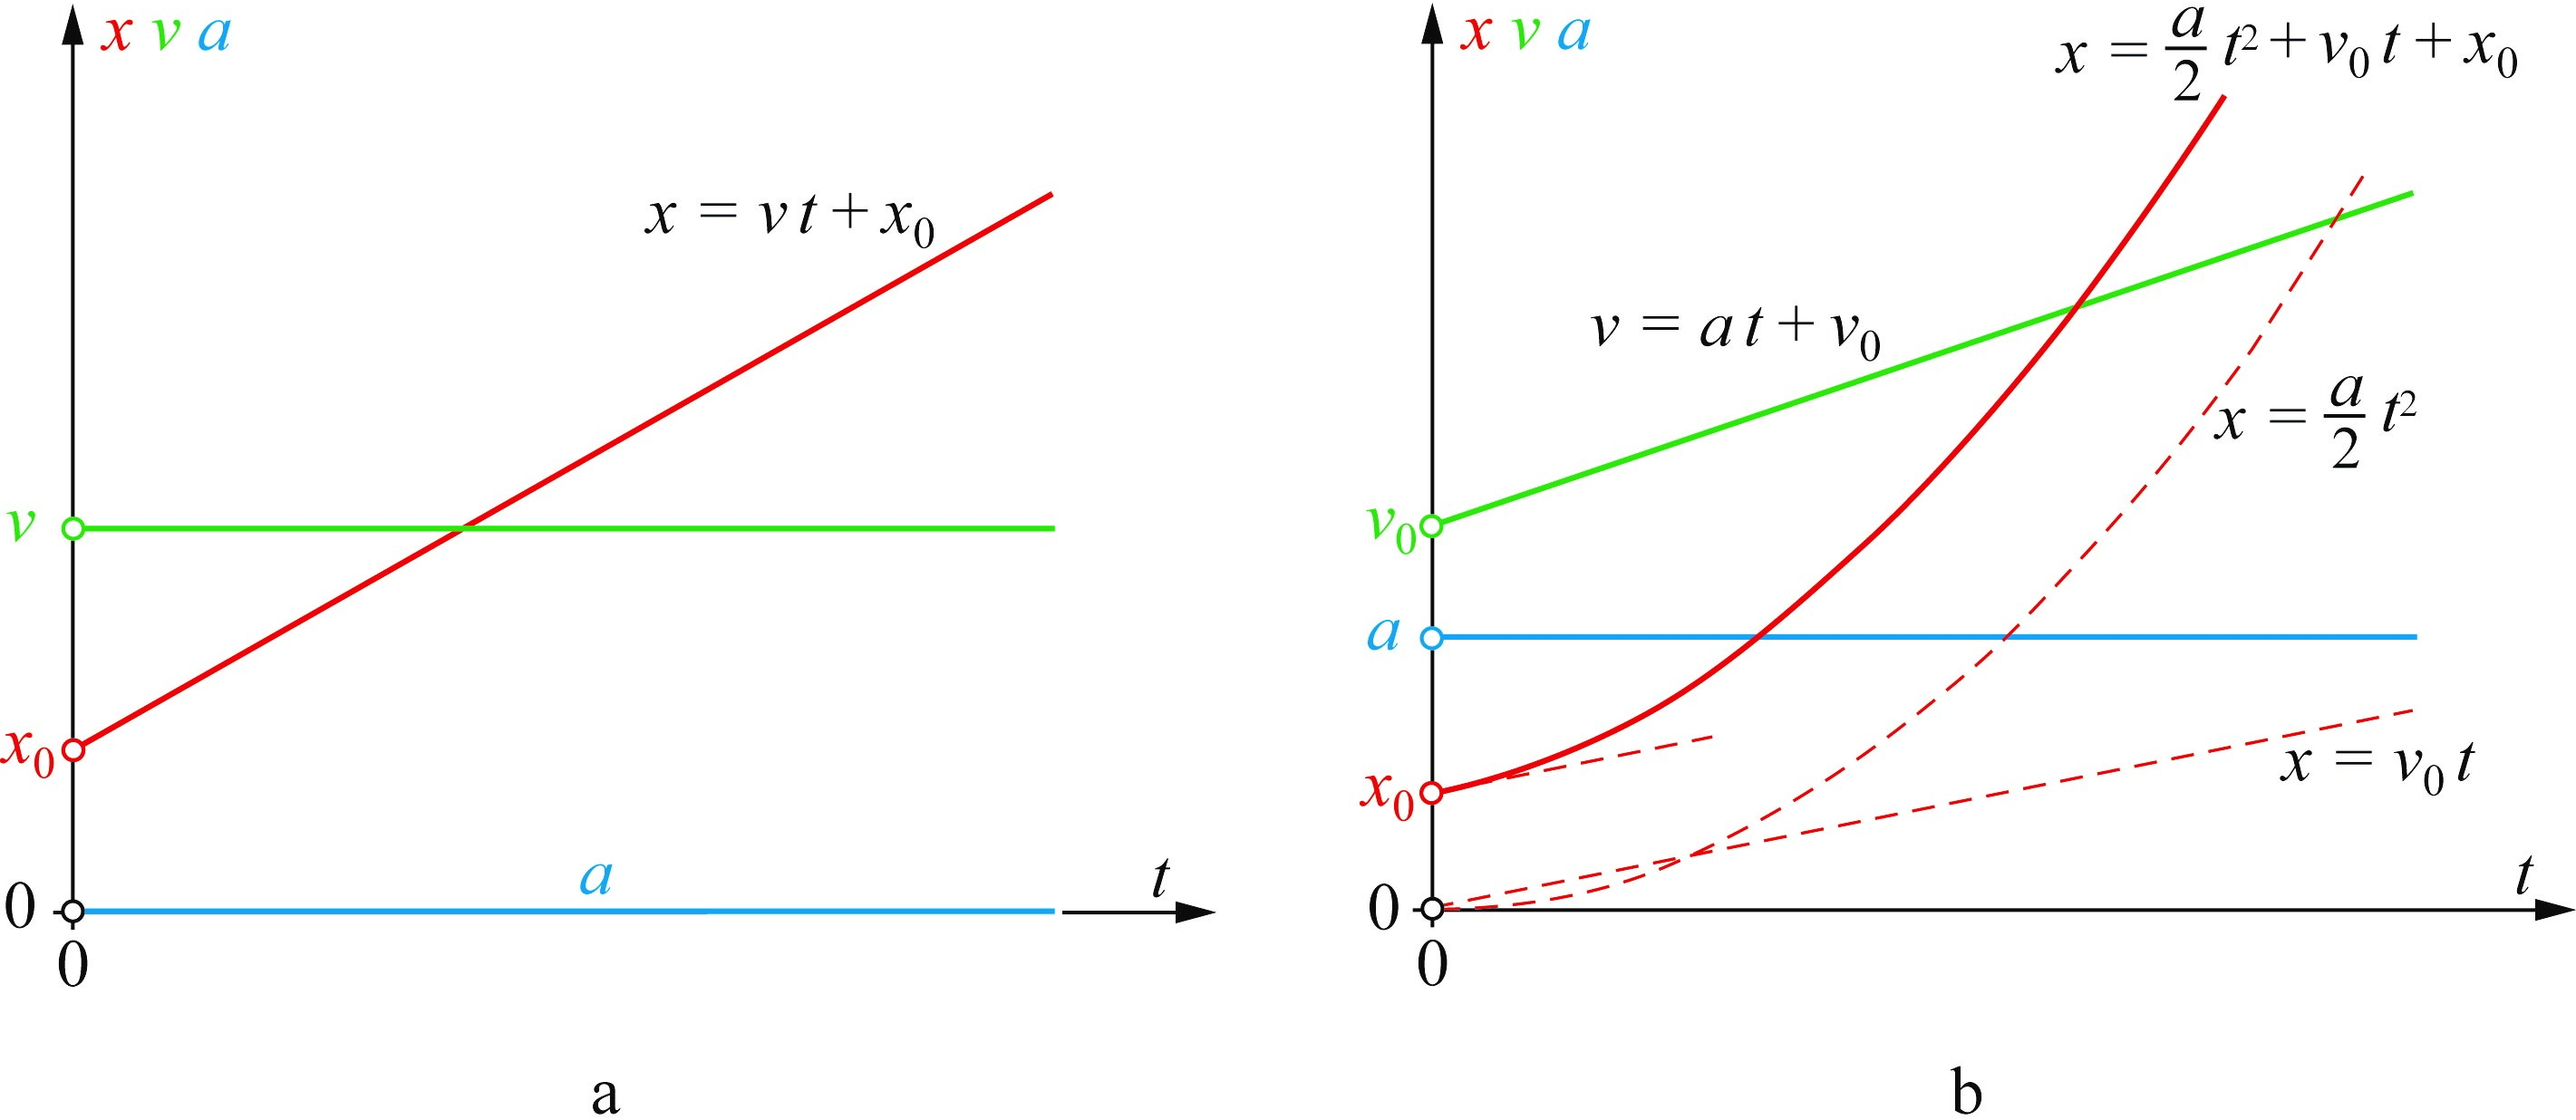
\includegraphics[width=0.9\linewidth]{img/kinematik1}
		
		\subsection{v-t Diagramme}
		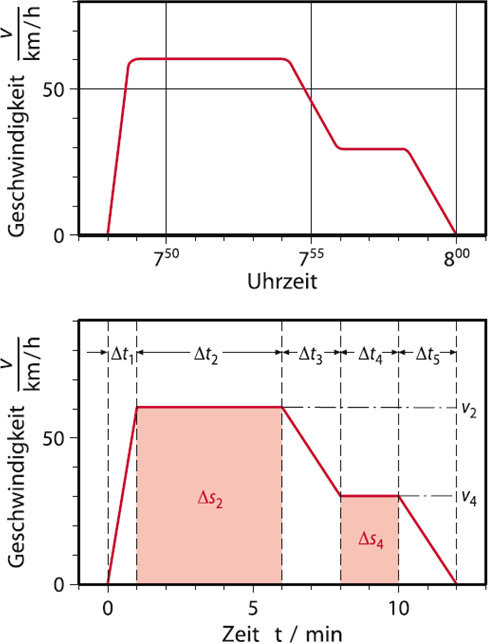
\includegraphics[width=0.9\linewidth]{img/v-t_diagram}
	\end{multicols}



\section{Kinetik}
	\begin{tabu} {l X l}
		\hline
		Impuls
		&	$\vec{p} = mv = \left[ Ns \right] = \left[ \frac{kg \cdot m}{s} \right]$
		& 
		\\ \hline
		Kraft
		&	$\vec{F}= m\vec{a} = \abl{\vec{p}}{t} = \left[ N \right] = \left[ \frac{kg \cdot m}{s^2} \right]$
		&	Newton
		\\ \hline
		Energie
		&	$W = F s \left[ J \right] = \left[ N m \right] = \left[ Ws \right] = \left[ \frac{kg \cdot m^2}{s^2} \right]$
		&	Joule
		\\
		Arbeit
		&	$1 \left[kWh\right] = 3.6 \cdot 10^6 \left[ J \right]$
		&
		\\ \hline
		Leistung
		&	$P = \abl{W}{t} = \left[ W \right] = \left[ \frac{J}{s} \right] = \left[ \frac{kg \cdot m^2}{s^3} \right] = Fv$ (bei Translation)
		&	Watt
		\\ \hline
	\end{tabu}
	
\subsubsection{Kinetische Energie}
	\begin{tabu} {l X}
		Kraft & $\vec{F} = m\vec{a} = \frac{\vec{p}}{t}$ \\
		Strecke & $s = \frac{1}{2} a t^2 + \vec{v}_0 \cdot t + s_0$ \\
		Geschwindigkeit & $\vec{v} = \vec{a}t + \vec{v}_0$ \\
		Beschleunigung & $\vec{a}$\\
		Impuls & $\vec{p} = m\vec{v}$ \\
		Energie & $W = E_{kin} Fs = \frac{1}{2} mv^2$
	\end{tabu}

\subsubsection{Potentielle Energie}
	
	\begin{tabu} {l X}
		Kraft & $\vec{F} = m\vec{g} = \frac{\vec{p}}{t}$ \\
		Höhe & $h = \left[ m \right]$ \\
		Geschwindigkeit & $\vec{v} = \vec{g}t$ \\
		Beschleunigung & $\vec{g} \approx 9.81 \frac{m}{s^2}$ \\
		Impuls & $\vec{p} = m\vec{v}$ \\
		Energie & $W = E_{pot} = Fh = mgh$
	\end{tabu}

\subsubsection{Federkraft}
	
	\begin{tabu} {l X}
		Federkonstante & $k = \left[ \frac{N}{m} \right] = \left[ \frac{kg}{s^2} \right]$ \\
		Kraft & $F = kx$ \\ %TODO: Was ist $x$? Stimt das? Siehe vier Zeilen weiter.
		Energie & $	W = E_f = \frac{1}{2} k x^2$
	\end{tabu}

	Die Ausdehnung von Federn ist proportional zur Kraft: $F = -k(x -x_0)$ %TODO: Stimmt diese Formel?

\subsection{Mehrdimensionale Kräfte}
\paragraph{Zweite Dimension} \hfill \\
	\begin{tabu} {l X}
		$F_x = $ & $F\cos(\alpha)$ \\
		$F_y = $ & $F\sin(\alpha)$ \\
	\end{tabu}

\pagebreak

\paragraph{Dritte Dimension} \hfill \\
	\begin{multicols}{2}
		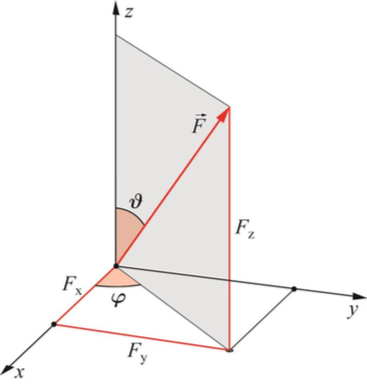
\includegraphics[width=0.6\linewidth]{img/darstellungKraefte.png}
		
		\begin{tabu} {l X}
			$\vec{r}(t) =$ & $ \left[ x(t),y(t),z(t)\right]$ \\
			$\vec{v}(t) =$ & $\frac{\text{d}\vec{r}}{\text{d}t}$ \\
			$F_x = $ & $F\cos(\varphi)\sin(\vartheta)$ \\
			$F_y = $ & $F\sin(\varphi)\sin(\vartheta)$ \\
			$F_z = $ & $F\cos(\vartheta)$
		\end{tabu}
	\end{multicols}

\subsection{Würfe}
\subsubsection{Senkrechter Wurf}
	\begin{multicols}{2}
		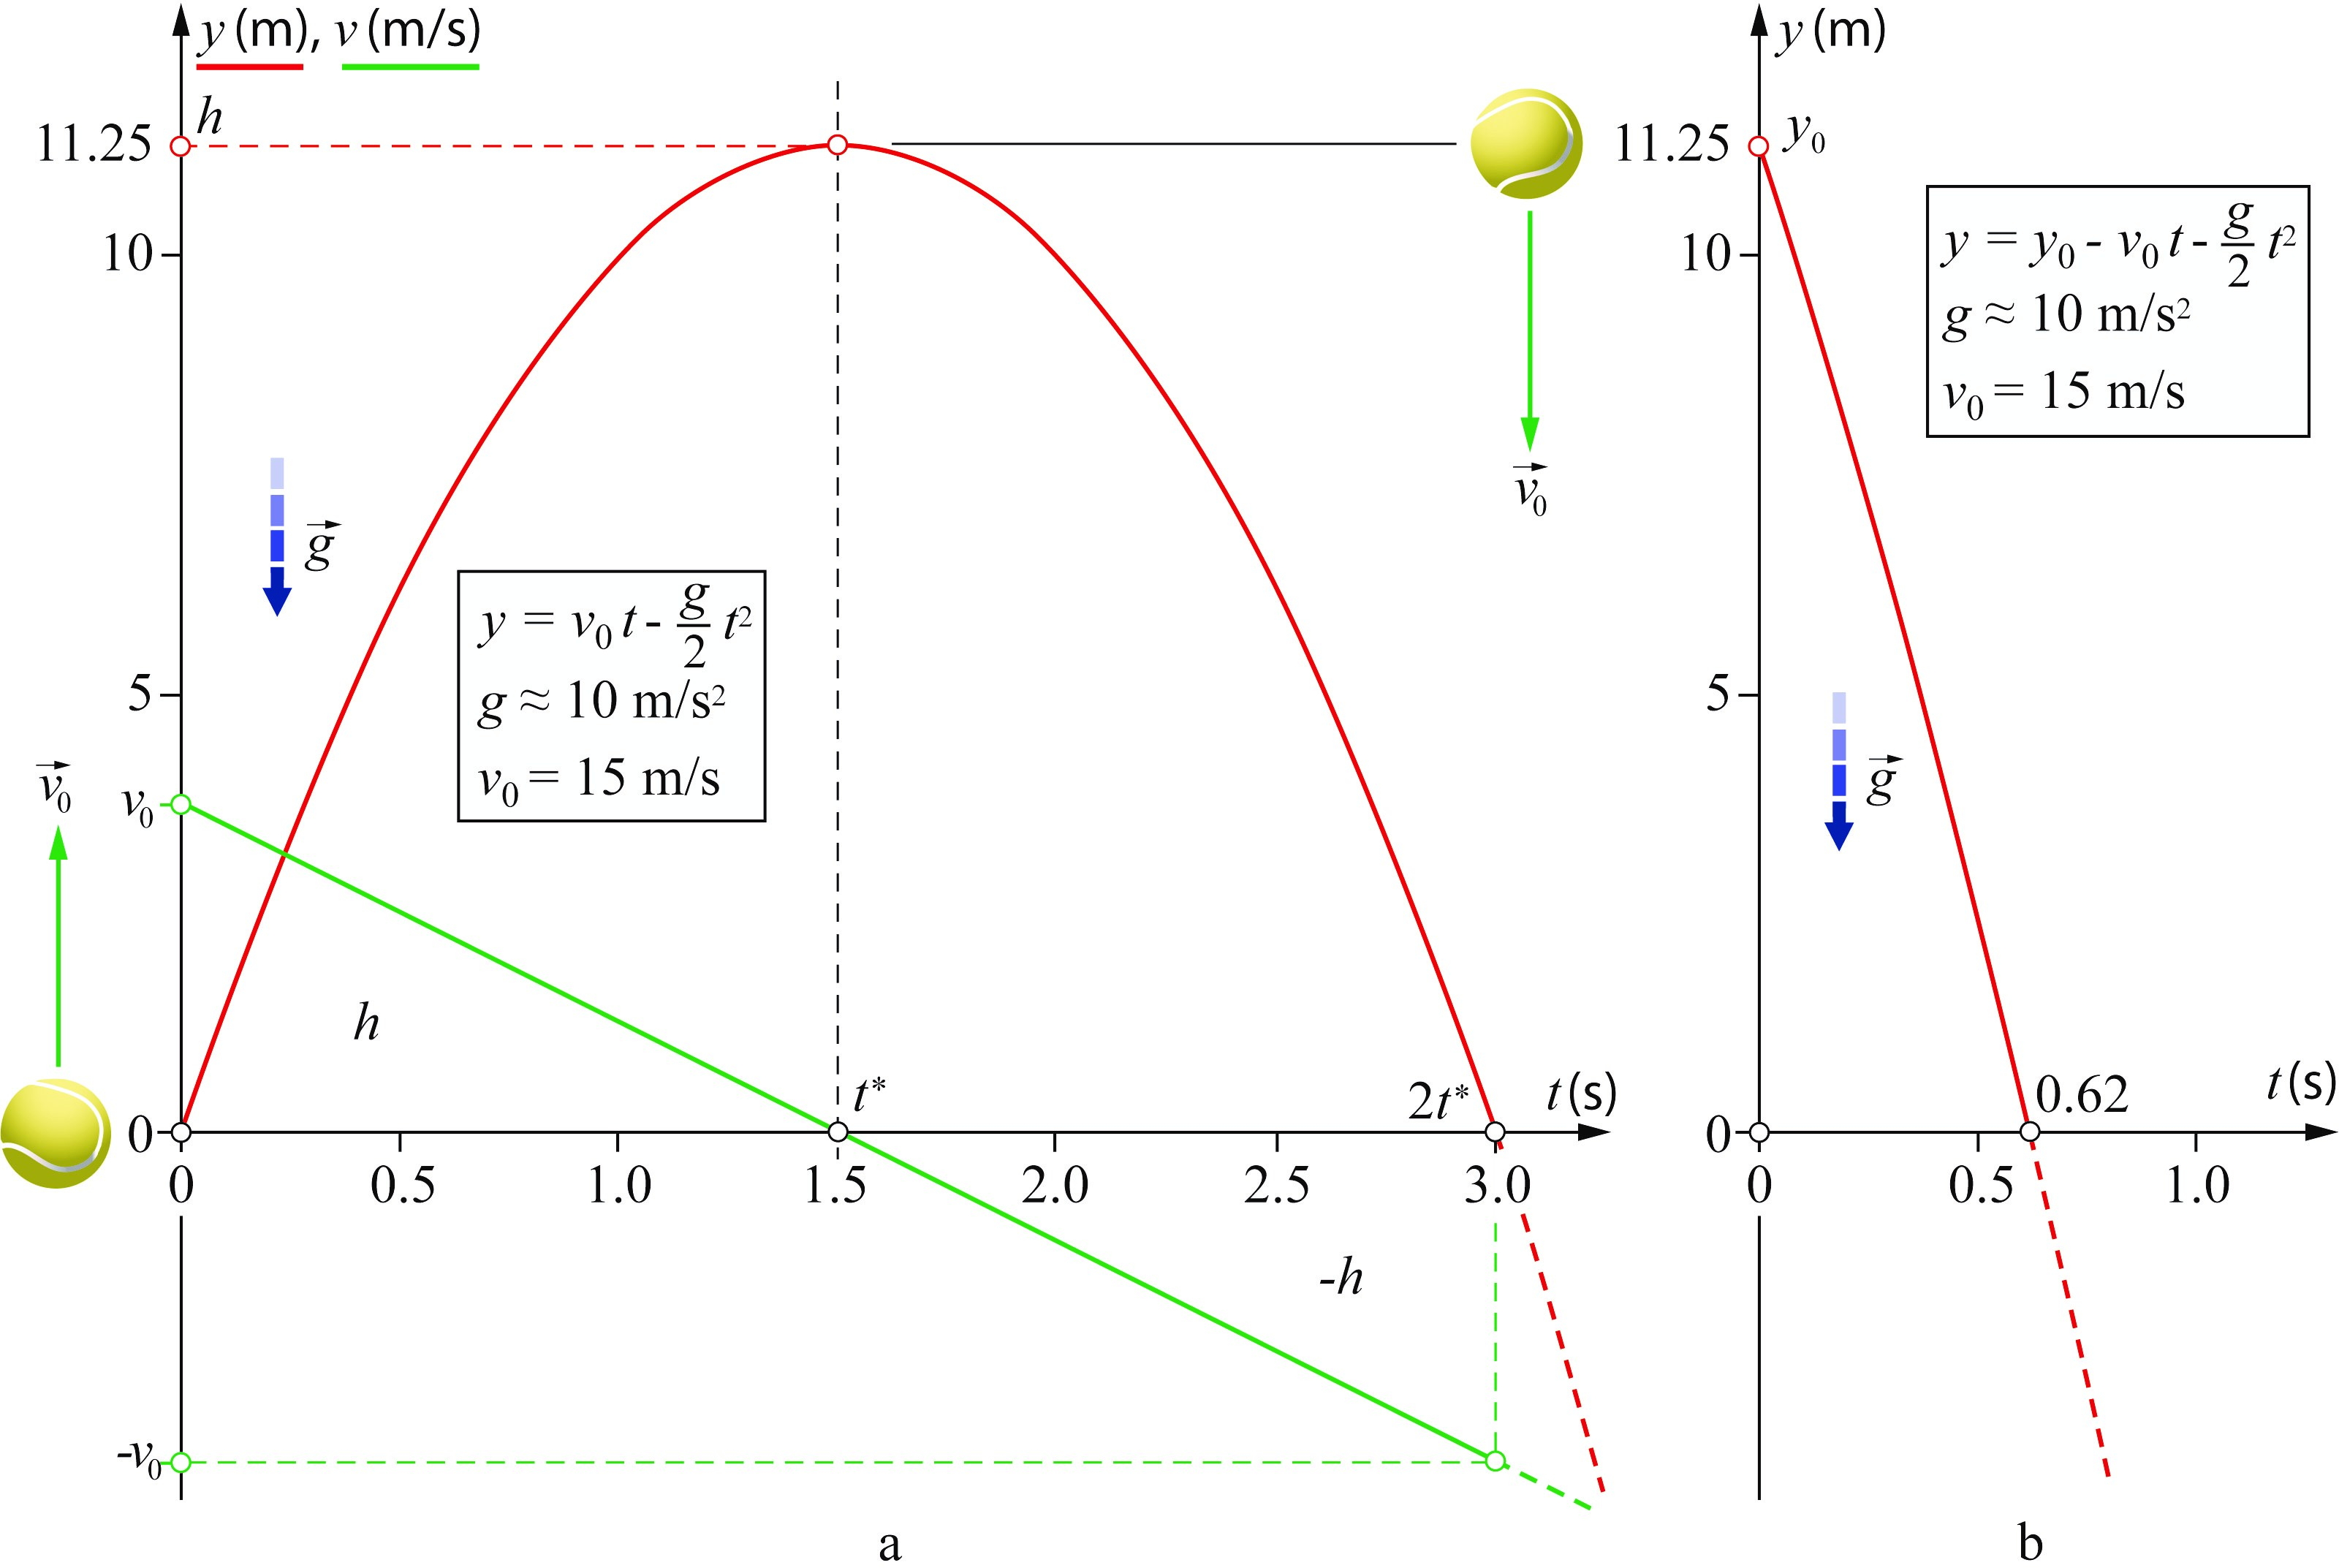
\includegraphics[width=\linewidth]{img/wurf_senkrecht}
		
		\begin{tabu} {l X}
			Maximale Wurfhöhe & $h = \frac{v^2_0}{2g}$
		\end{tabu}
	\end{multicols}

\subsubsection{Horizontaler Wurf}
	\begin{multicols}{2}
		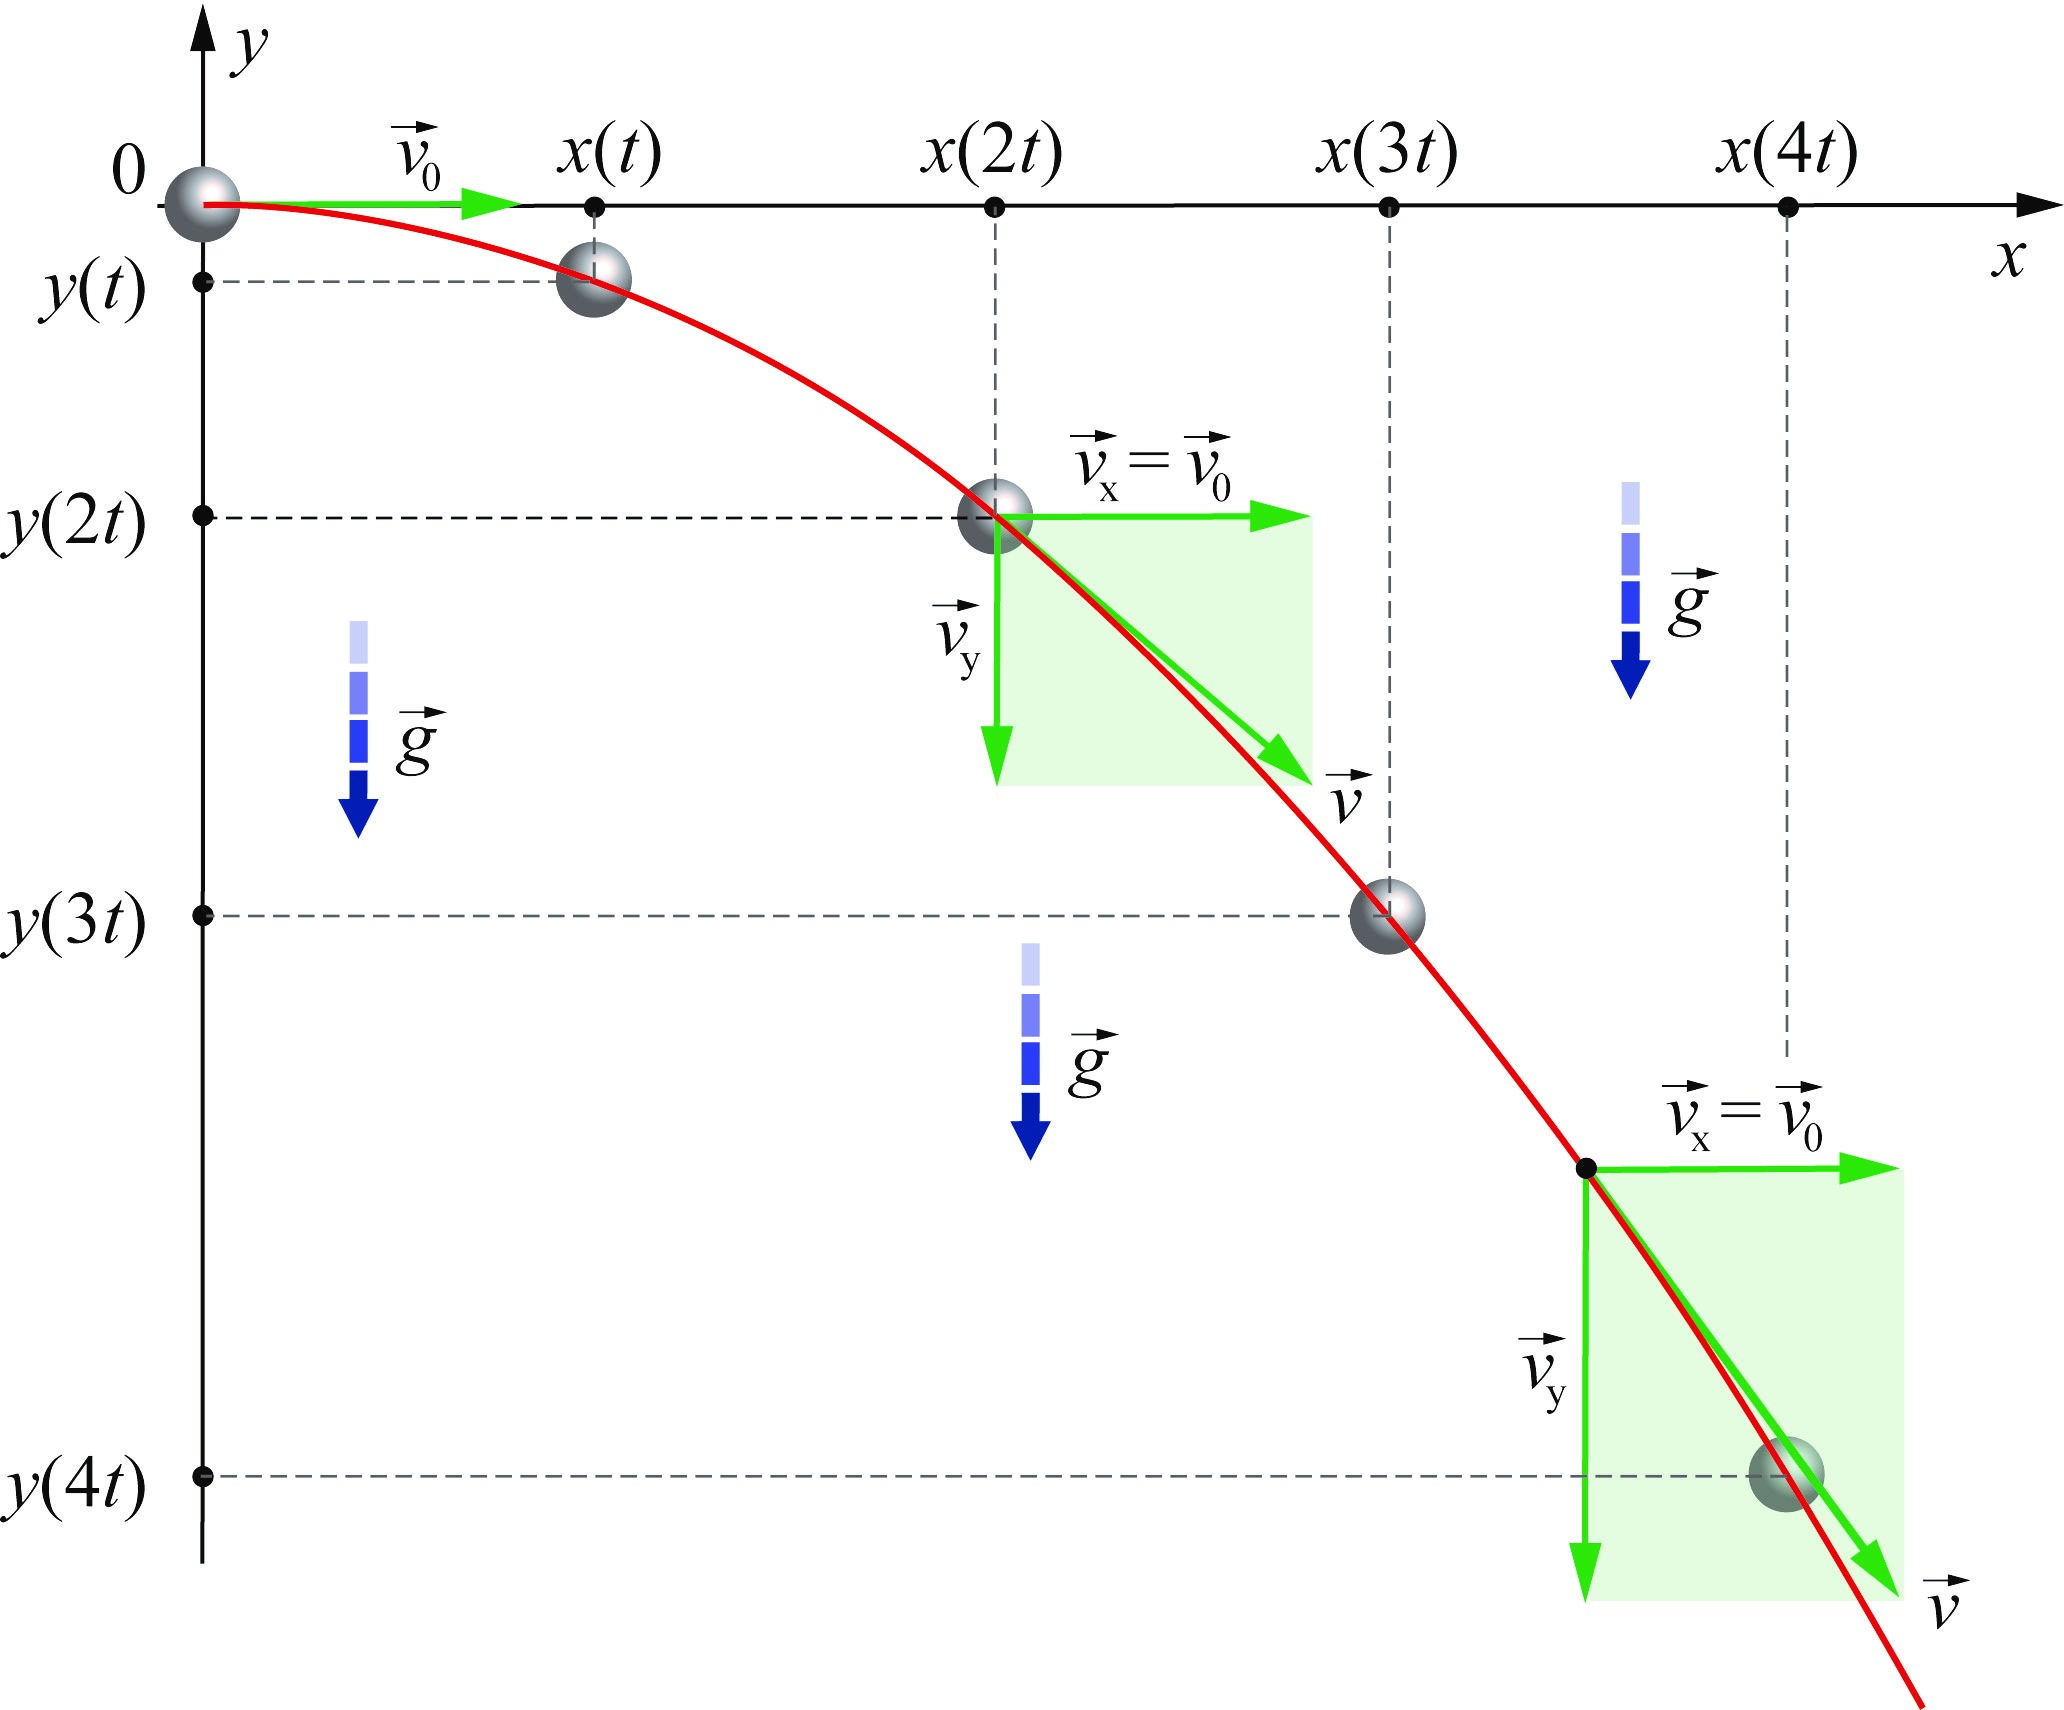
\includegraphics[width=\linewidth]{img/wurf_horizontal}
		
		\begin{tabu} {l X}
			Strecke & $x = v_0 t$ \\
			Zeit & $t = \frac{x}{v_0}$ \\
			Höhe & $y = - \frac{g}{2}t^2 = - \frac{g}{2v^2_0} x^2$
		\end{tabu}
	\end{multicols}

\subsubsection{Schiefer Wurf}
	\begin{multicols}{2}
		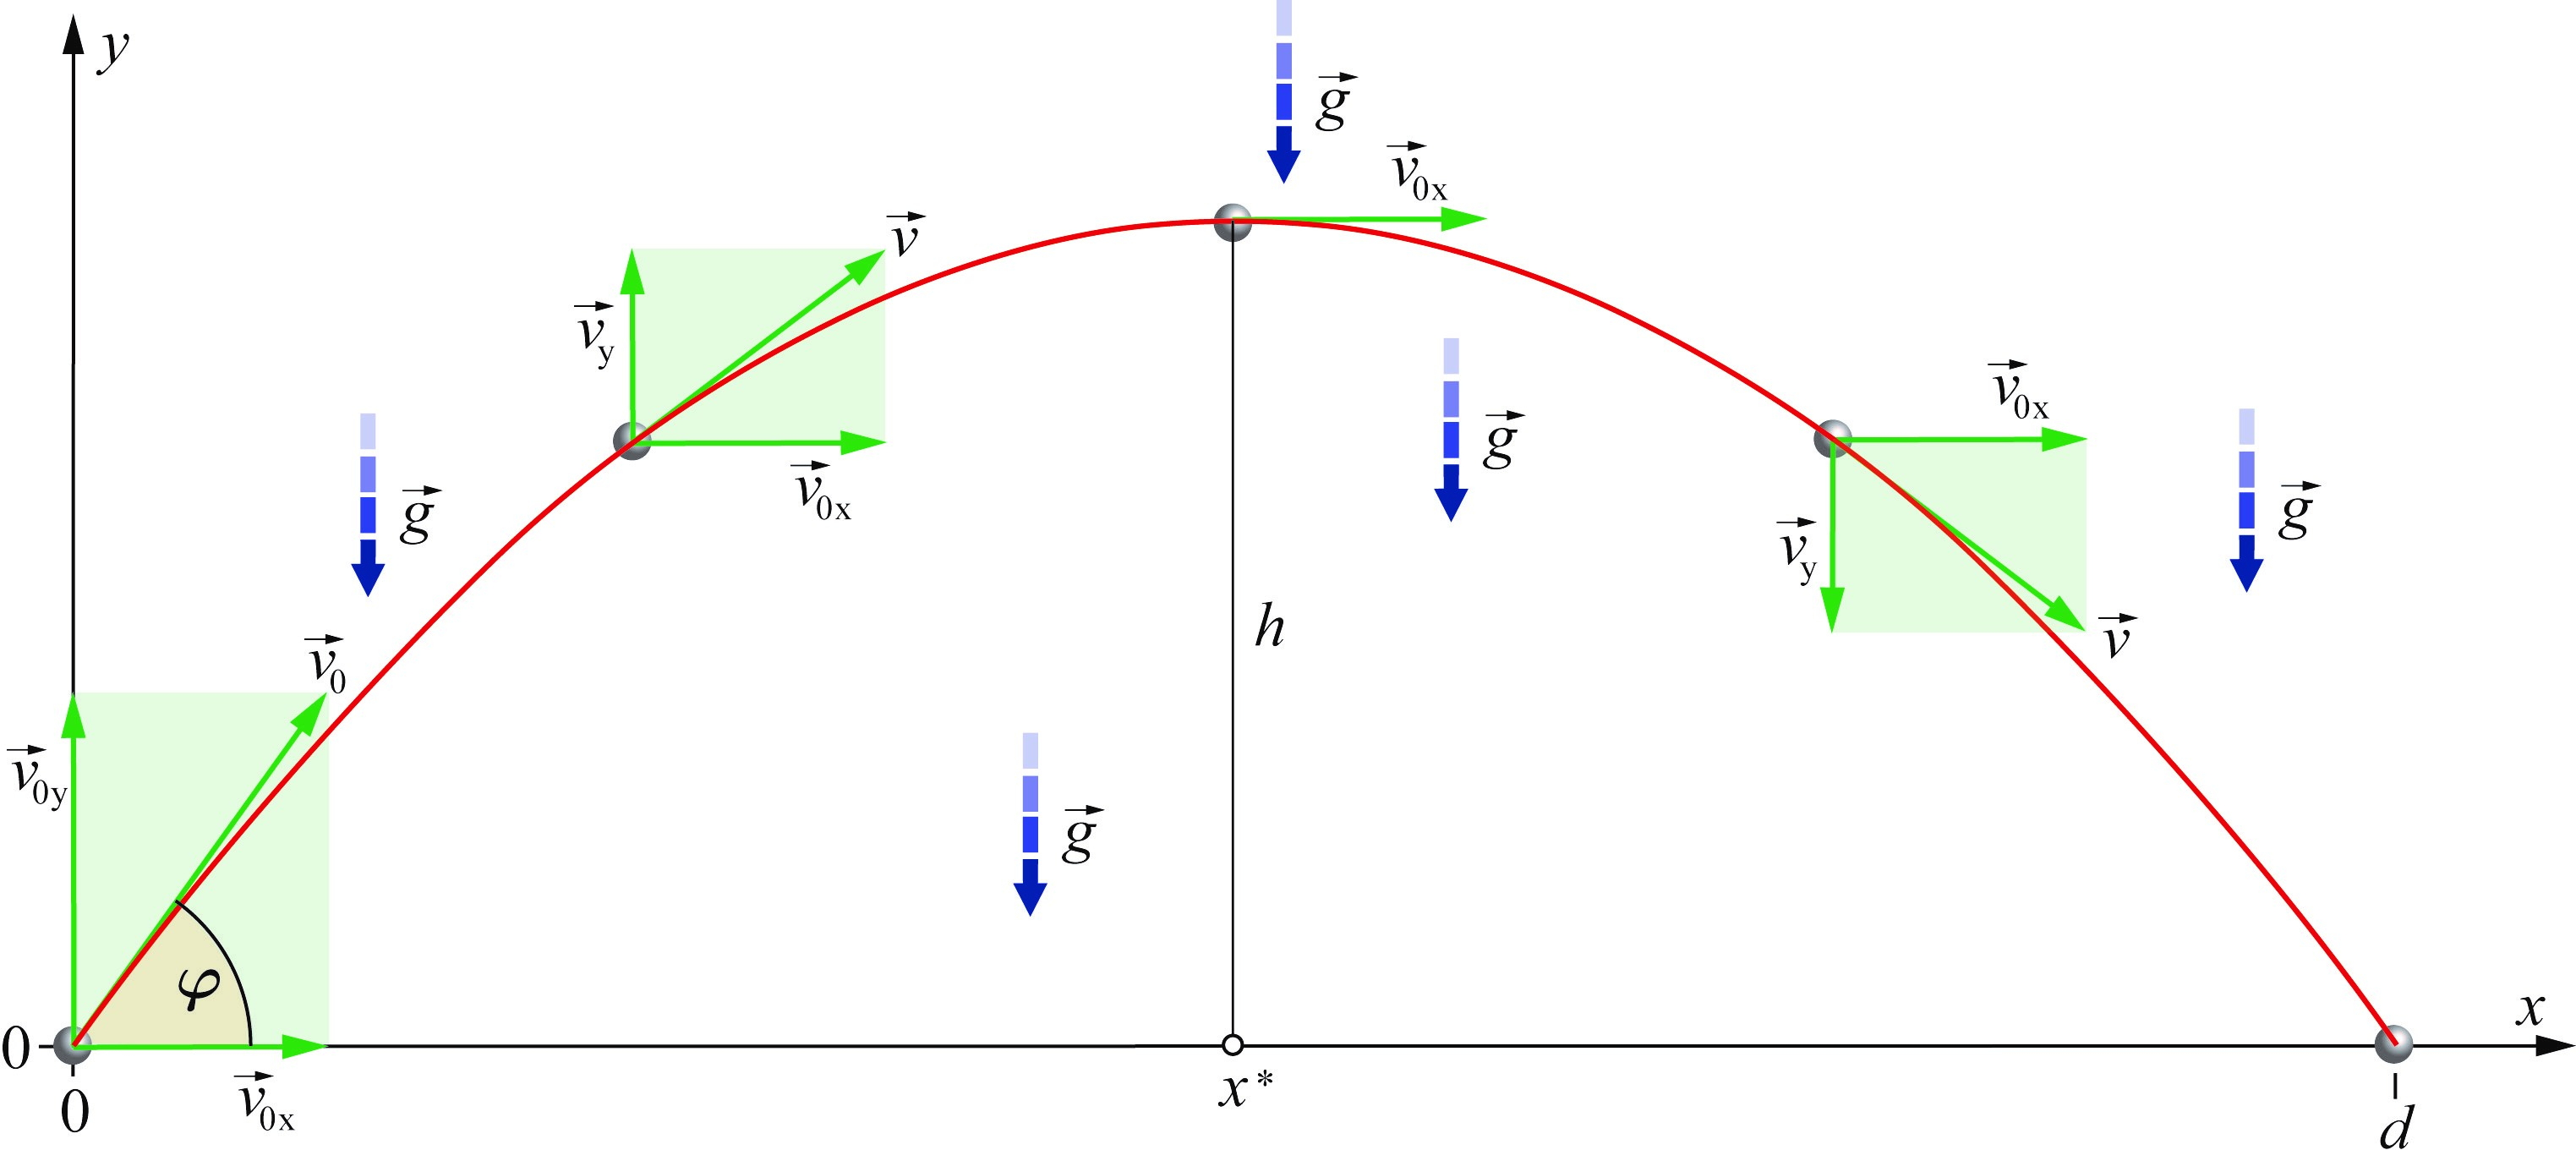
\includegraphics[width=\linewidth]{img/wurf_schief}

		\begin{tabu} {l X}
			Höhe & $y(x) = x \tan \varphi - \frac{g x^2}{2 v^2_0 \cos^2 \varphi}$ \\
			Max. h. & $y_{max} = \frac{v^2_0 \sin^2 \varphi}{2g}$ \\
			Wurfweite & $d = \frac{v^2_0 \sin(2\varphi)}{g}$
		\end{tabu}
	\end{multicols}

\subsection{Haft- und Gleitreibung}
	Ist immer unabhängig von der Fläche.
	
	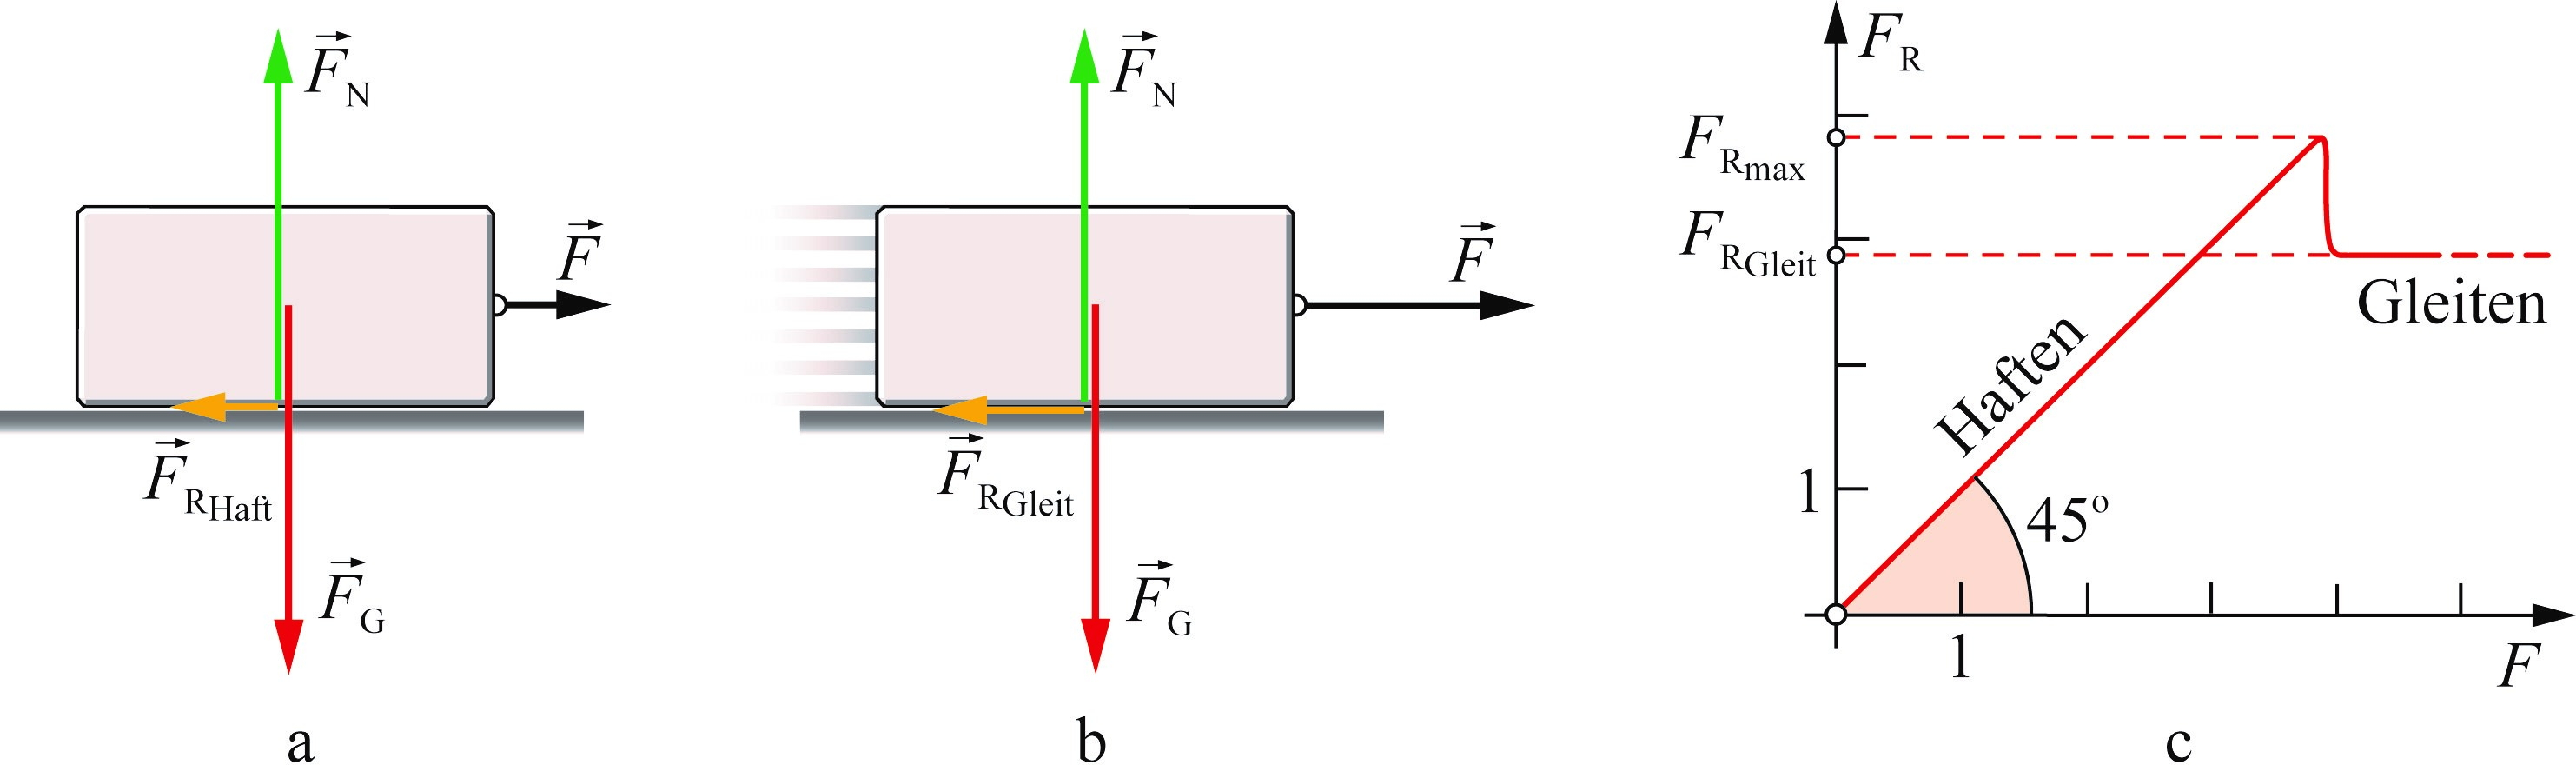
\includegraphics[width=\linewidth]{img/reibung}
	
	\begin{tabu}{l X}
		Maximale Haftreibung & $F = F_{R,max} = \mu_H F_N$\\
		Gleitreibung & $F = \mu_G F_N$
	\end{tabu}
	
\subsubsection{Schiefe Ebene}
	\begin{multicols}{2}
		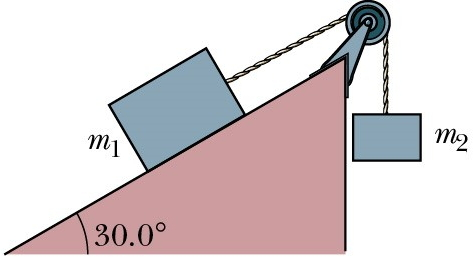
\includegraphics[width=\linewidth]{img/reibung_schiefe_ebene.jpg}
		
		\begin{align*}
			F_N &= m_1 g \cos 30^\circ \\
			m_1 &g \sin 30^\circ - m_2 g \pm \mu_Hm_1g \cos 30^\circ = 0
		\end{align*}
	\end{multicols}

\subsubsection{Beispiel für zwei Dimensionen}
	\begin{multicols}{2}
		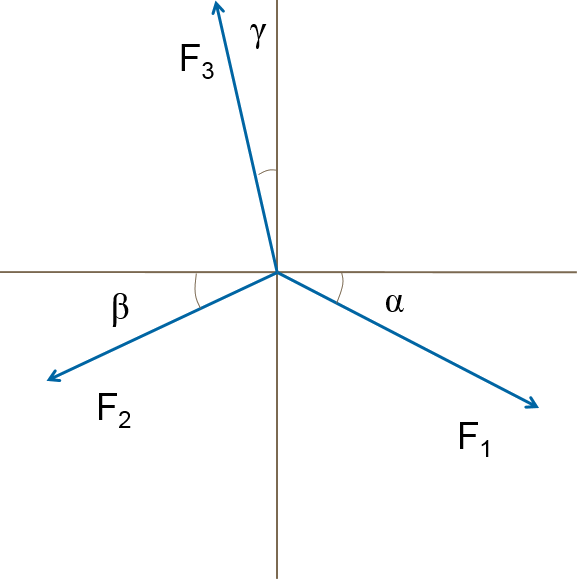
\includegraphics[width=0.5\linewidth]{img/massenpunkt}
		
		\begin{tabu}{l X}
			X: & $F_1 \cos \alpha - F_2 \cos \beta - F_3 \sin \gamma = 0$\\
			Y: & $-F_1 \sin \alpha - F_2 \sin \beta + F_3 \cos \gamma = 0$
		\end{tabu}
	\end{multicols}


\subsection{Gleichgewicht eines starren Körpers an der Ebene}	
	Die Summe der Kräfte muss gleich 0 sein, und mittels Vektoraddition anhand eines Referenzpunktes ausgerechnet werden:
	
	\[
	\vec{F}_{tot} = \vec{M}_{tot} = \sum_n{\vec{F}_n} =\sum_n{\vec{F}_{x,n}} = \sum_n{\vec{F}_{y,n}} = \sum_n{\vec{F}_{z,n}} = 0
	\]

%TODO: Slide 26 Vorlesung

\subsubsection{Schwerpunkt}
	Wird der Körper am Schwerpunkt aufgehängt, ist er im Gleichgewicht, d.h., Drehmoment = 0. Die Schwerkraft kann durch eine Kraft im Schwerpunkt ersetzt werden:
	\[
		r_p \sum_i{m_i} = \sum_i{m_ir_i} %TODO: Versteh ich nicht. Was ist hier r und m?
	\]

\pagebreak

\subsection{Dynamik}
	\begin{multicols}{2}
		\begin{align*}
		Ma &= Mg - F_s \\
		ma &=F_s - mg
		\end{align*}
		
		Daraus folgt: $(m + M)a = g(M - m)$
		
		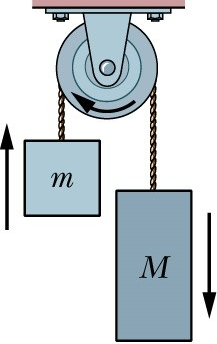
\includegraphics[width=0.3\linewidth]{img/dynamik}
	\end{multicols}

\subsection{Arbeit und Energie}
\subsubsection{Beispiel Bungee Jumping}
	\begin{multicols}{2}
		Kehrpunktgeschwindigkeit = 0
		\begin{align*}
			mg(L + d) = \frac{k}{2} d^2 + \frac{m}{2} v^2\\
			d^2 - \frac{2mg}{k}d - \frac{2mg}{k}L = 0\\
			d = \frac{mg}{k} + \sqrt{\frac{2mg}{k} + \left(\frac{mg}{k}\right)^2}
		\end{align*}
		

		
		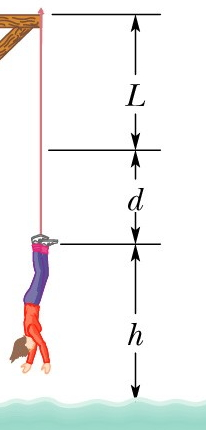
\includegraphics[width=0.25\linewidth]{img/bungee}
	\end{multicols}

\subsection{Leistung}
	\begin{tabu}{l X}
		Wirkungsgrad & $\eta = \frac{P_\text{nutzbar}}{P_\text{zugeführt}} < 1$
	\end{tabu}

\subsection{Rotation}
	\begin{tabu} {l X}
		Periode
		& $T = \left[ s \right]$ (Zeit einer Umdrehung) \\
		Frequenz
		& $f = T^{-1} = \left[ s^{-1} \right]$ \\
		Winkelgeschwindigkeit
		& $\vec{\omega} = 2\pi f = \frac{2\pi}{T} = \left[ \frac{rad}{s} \right]$ \\
		Winkelbeschleunigung
		& $\vec{\alpha} = \abl{\vec{\omega}}{t} = \left[ \frac{rad}{s^2} \right]$ \\
		Rotationsgeschwindigkeit
		& $v = \omega r = \frac{2\pi r}{T} = \left[ \frac{m}{s} \right]$ \\
%TODO: Was ist die Tangentialbeschleundigung? Stimmt die Formel?
%		Tangential- und 
%		& $\vec{a}(t) = \vec{a}_t(t) + \vec{a}_r(t)$ \\
		Radialbeschleunigung
		& $a_r = \omega^2 r = \frac{v^2}{r} = \left[ \frac{m}{s^2} \right]$ \\
		Rotationsenergie
		& $W = E_{rot} = \frac{1}{2} J \omega^2 = \left[ J \right]$ \\
		Rotationsleistung
		& $P = \vec{M} \cdot \vec{\omega} = \left[ \frac{J}{s} \right]$ \\
		Drehimpuls
		& $\vec{L} = J \vec{\omega} = \left[ \frac{kg \cdot m^2}{s} \right]$ \\
		Drehmoment / Kraft
		& $\vec{M} = \vec{r} \times \vec{F} = \abl{\vec{L}}{t} = \left[ Nm \right]$ (siehe \ref{sec:drehmoment} Drehmoment) \\
		Massenträgheitsmoment
		& $J = \sum_i{m_i r_i^2} = \left[kg \cdot m^2 \right]$
	\end{tabu}

\subsubsection{Radialbeschleunigung}
	Die Radialbeschleunigung zeigt nach innen zum Kreismittelpunkt

\subsubsection{Rotationsenergie}

	%TODO: Slide 3, Freitag 21.04.


\subsubsection{Drehmoment}\label{sec:drehmoment}
	\begin{multicols}{2}
		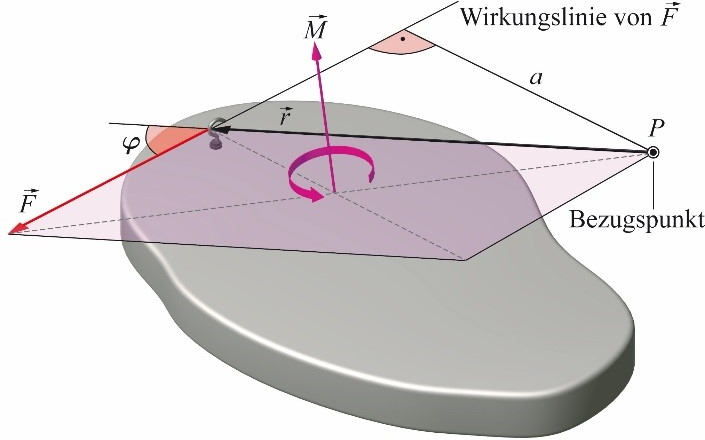
\includegraphics[width=0.9\linewidth]{img/drehmoment}
		
		\begin{align*}
		M &= a \cdot F \\
		\vec{M} &= \vec{r} \times \vec{F} \\
		\left| \vec{M} \right| &= \left| \vec{r} \right| \left| \vec{F} \right| \sin \varphi
		\end{align*}
		
		Der Drehmoment wird in $t^{-1}$, meist $\text{s}^{-1}$ oder $\text{min}^{-1}$ angegeben.
	\end{multicols}

\subsubsection{Hebelkraft}
	\begin{multicols}{2}[Hebelkraft funktioniert dank dem Drehmoment.]
		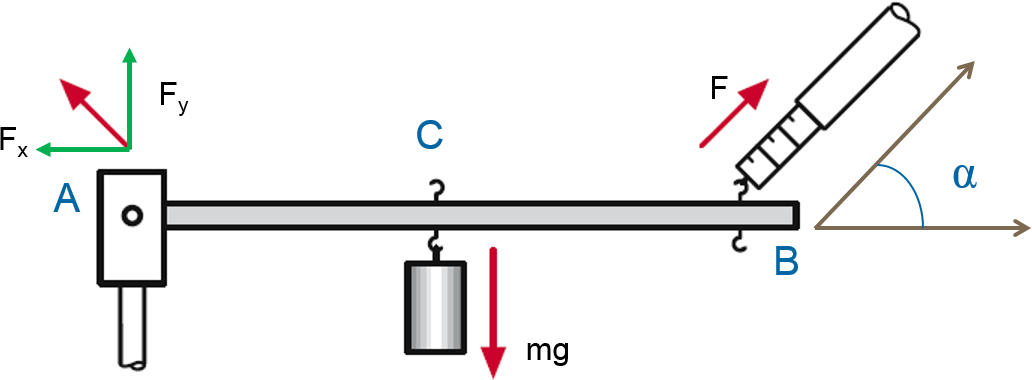
\includegraphics[width=\linewidth]{img/hebelkraft}
		Gegeben: $\alpha$ und $mg$. Gesucht: $F$.
		
		\begin{tabu}{l X}
			X: & $F \cos \alpha - F_x = 0$\\
			Y: & $F \sin \alpha + F_y - mg = 0$\\
			M$_z$ & $F \sin \alpha \cdot L - mg \frac{L}{2} = 0$
		\end{tabu}
		Daraus folgt: $F = \frac{mg}{2 \sin \alpha}$
	\end{multicols}

\subsection{Impuls}

Impulserhaltung: In einem geschlossenen System ohne externe Einflüsse ist der Impuls 0. Wenn nur Kräfte zwischen zwei Körpern wirken (Kraft=Gegenkraft), bleibt der Impuls erhalten
	
\subsubsection{Drehimpuls}
	Der Drehimpuls $L$ ist parallel zur Drehachse. Um diesen zu ändern, braucht es einen Drehmoment.

	\[
	%TODO: Stimmt der hintere Teil oder nicht?
	L = J \omega %= \sum_i{r_i \times p_i} = \sum_i{r_i \times mv_i} = \left[ \frac{kg \cdot m^2}{s^2} \right]
	\]
	
	Dynamisches Gesetz der Rotation:
	$\abl{L}{t} = M$
	
	 Wenn keine externe Momente wirken, bleibt der Gesamtdrehimpuls konstant.
	%TODO: Screenshot Slide 8
	
	\paragraph{Drehimpuls auf der schiefen Ebene} \hfill \\
	
	Runde Zylinder, welche eine schiefe Ebene hinunter rollen: $mgh = E_{kin} + E_{rot} =\frac{m}{2} v^2 + \frac{J}{2} \omega^2$
	
	Je weiter die Masse von der Drehachse weg ist, desto träger ist die Drehung.

\subsection{Masse und Trägheit}
	Das Gewicht eines Körpers ist von der Masse abhängig: $F = mg$.
	Masse ist für eine Trägheit und Gravitation zuständig. Achtung: Gewicht $\neq$ Masse!
	%TODO: Erweitern Masse und Trägheit

\subsubsection{Trägheitsmoment}

	%TODO: Slide 5 21.4.
	
	Bezüglich einer Achse:
	
	$J = \int r^2 d m = \left[ kg \cdot m^2 \right]$

\subsection{Stösse}
	
	Geschwindigkeit des Schwerpunktes:
	\begin{align*}
		 u &= \frac{m_1v_1 + m_2v_2}{m_1 + m_2}
	\end{align*}
	
	Vor dem Stoss:
	\begin{align*}
		v_1 &= u + (v_1 - u) = u + v_1^{rel} \\
		v_2 &= u + (v_2 - u) = u + v_2^{rel}
	\end{align*}
	
	Kinetische Energie:
	\begin{align*}
		E_{kin} &= \frac{m_1 + m_2}{2}u^2 + \frac{m_1}{2}(v_1 - u)^2 + \frac{m_2}{2}(v_2 - u)^2
	\end{align*}
	
\subsubsection{Elastischer Stoss}
	Sowohl Impuls als auch Kinetische Energie bleibt erhalten.
	
	Nach dem Stoss:
	\begin{align*}
	v_1 &= u - (v_1 - u) = u - v_1^{rel} \\
	v_2 &= u - (v_2 - u) = u - v_2^{rel}
	\end{align*}

\subsubsection{Inelastischer Stoss}
	Nach dem Stoss: $v_1 = v_2 = u$

	Kinetische Energie:
	\begin{align*}
		E_{kin} &= m_1 v_1 + m_2 v_2 = (m_1 + m_2) u \Rightarrow u = \frac{m_1 v_1 + m_2 v_2}{m_1 + m_2}
	\end{align*}

\subsubsection{Verlorene Kinetische Energie}
	\begin{align*}
		Q &= E_{kin}  - E'_{kin}
	\end{align*}

\subsubsection{Kraftstoss}

	$\int\limits^{t_2}_{t_1} p(t) dt = p(t_2) - p(t_1) = \int\limits^{t_2}_{t_1} F(t) dt$


\section{Hydrostatik}
	\begin{tabu} {l X l}
		\hline
		Druck
		&	$p = \frac{F}{A} = \left[ Pa \right] = \left[ \frac{N}{m^2} \right] = \left[ \frac{J}{m^3} \right] = \left[ \frac{kg}{m \cdot s^2} \right]$
		&	Pascal \\
		& $1 \text{ bar } = 10^5 Pa$ &
		\\ \hline
		Hydrostatischer Druck
		& $p = \rho g h$ & \\ \hline
		Dichte
		& $\rho = \frac{m}{V}$ &\\ \hline
		Kraft
		& $F = \frac{p}{A}$ & \\ \hline
		Fläche
		& $A = \left[ m^2 \right]$ & \\ \hline
		Masse & $m = \rho V = \rho A \Delta h = \left[ kg \right]$
	\end{tabu}

	\hfill \\
	In der Hydrostatik geht es um die Beschreibung von Fluiden, d.h. Flüssigkeiten und Gasen.


\subsection{Druck}
\subsubsection{Beispiel Schweredruck}
	\begin{multicols}{2}
		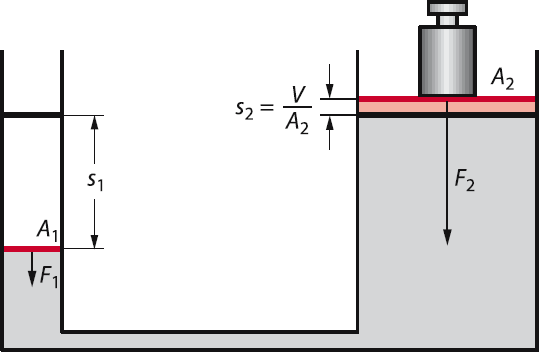
\includegraphics[width=\linewidth]{img/hydrostatik}
		
		\begin{align*}
			F_1 &= p A_1\\
			F_2 &= p A_2\\
			\frac{F_1}{A_1} = \frac{F_2}{A_2} &\Rightarrow F_2 = \frac{A_2 F_1}{A_1}
		\end{align*}	
	\end{multicols}

\subsection{Beispiel Hydrostatischer Druck}
	\begin{multicols}{2}
		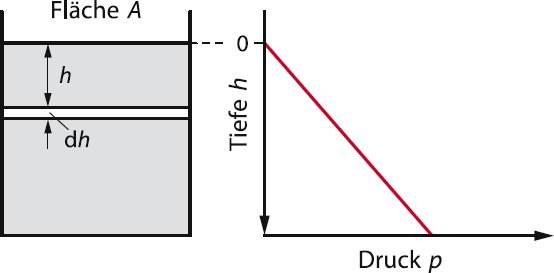
\includegraphics[width=\linewidth]{img/hydrostatischer_druck}
		
		\begin{align*}
		dp &= \rho \cdot g \cdot dh\\
		F_2 &= p A_2\\
		\frac{F_1}{A_1} = \frac{F_2}{A_2} &\Rightarrow F_2 = \frac{A_2 F_1}{A_1}
		\end{align*}	
	\end{multicols}


\subsection{Statischer Auftrieb}
	Das Gewicht des verdrängten Fluids geht verloren. Auftrieb: $F_A = \rho_f g V$
	
\subsubsection{Beispiel: Benötigte Seilkraft}
	\begin{multicols}{2}
		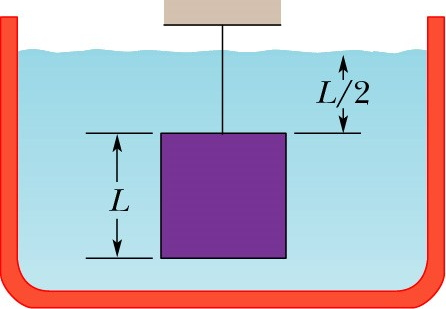
\includegraphics[width=\linewidth]{img/statischer_auftrieb.jpg}
		
		\begin{align*}
			F_s= mg - \rho_f V g = (\rho - \rho_f) V g
		\end{align*}
		
		Wenn die Dichte des Körpers kleiner als des Fluids ist, wird die Kraft negativ (Auftrieb)
	\end{multicols}


\subsection{Strömungen und Luftwiderstand}
\subsubsection{Kontinuitätsgleichung (Masenerhaltung)}
	\begin{multicols}{2}
		$u = v = $ Strömungsgeschwindigkeit \\
		Der Massenfluss einer Strömung ist erhalten. Somit gilt: \hfill \\
		$\dot{m} = \rho_1 v_1 A_1 = \rho_2 v_2 A_2 =  \left[ \frac{kg}{s} \right]$ \\
		Wenn die Dichte konstant ist, ist der Volumenstrom auch erhalten: \hfill \\
		$\dot{V} = v_1 A_1 = v_2 A_2$
		
		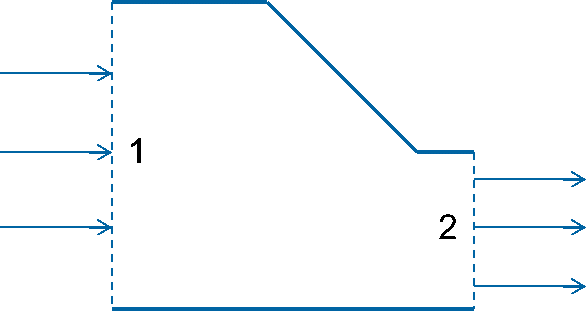
\includegraphics[width=0.9\linewidth]{img/kontinuitaetsgleichung}
	\end{multicols}
	
	\paragraph{Spezialfall: Inkompressibel} $\rho_1 = \rho_2$, Volumenstrom $V_1 A_1 = V_2 A_2$ mit $VA = \left[ m^2/s \right]$


\subsubsection{Energieerhaltung - Bernoulli}
	Der Totaldruck ist entlang einer Stromlinie erhalten:
	
	\begin{align*}
		p_1 + \frac{\rho}{2} v_1^2 + \rho g h_1 &= p_2 + \frac{\rho}{2} v_2^2 + \rho g h_2
	\end{align*}
	
	\paragraph{Typisches Beispiel} \hfill \\
	\begin{multicols}{2}[]
		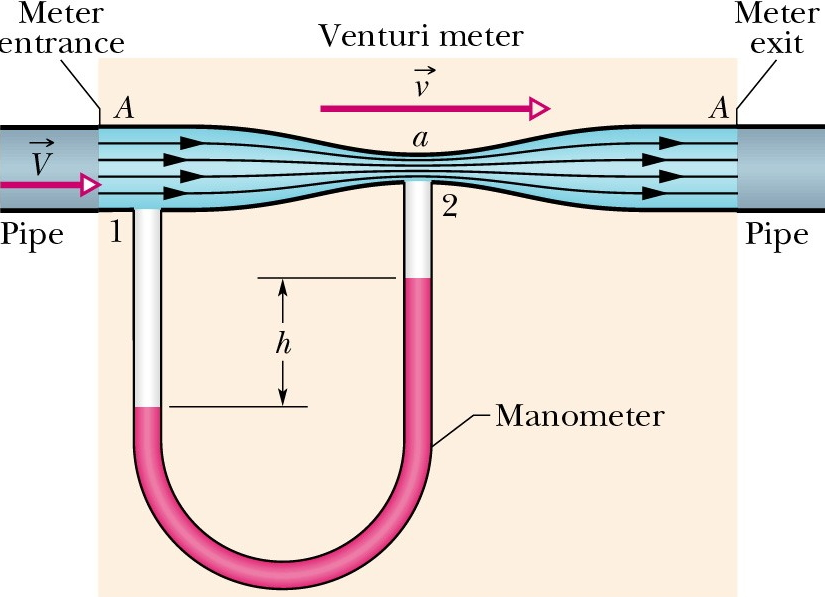
\includegraphics[width=\linewidth]{img/bernoulli}
		
		\begin{align*}
			V &= \sqrt{\frac{2a^2 \Delta p}{\rho (A^2 - a^2)}} = \sqrt{\frac{2 a^2 \rho_w g h}{\rho (A^2 - a^2)}}
		\end{align*}
	\end{multicols}


\subsubsection{Gesetz von Torricelli}
	\[
		v = \sqrt{2gh}
	\]
	Spezialfall der Bernoulli-Gleichung: Auslaufen aus einem Gefäss. $h$ ist der Fluidhöhe ab Auslauf, $v$ die Ausflussgeschwindigkeit.
	

\subsubsection{Turbulenzen - Reynolds-Zahl}
	Die Reynolds-Zahl besangt, wann eine Strömung nicht mehr laminar ($<2400$) sondern turbulent ($>2400$) wird.
	
	\[
		Re = \frac{\rho v D}{\mu}
	\]

	\begin{description}
		\item[$\rho$] Dichte
		\item[v] Geschwindigkeit
		\item[D] Durchmesser
		\item[$\mu$] Dynamische Viskosität (Einheit: $Pa \cdot s = \frac{kg}{m \cdot s}$)
	\end{description}

%DONE until here (until and with Page 12)









Avogadro Konstante: $N_A \approx 6.022 \cdot 10^23 Teilchen$

Die Knudsen Zahl: $Kn = \frac{\lambda}{L} \ll 1$

Dichte eines Fuluidelements: $\varrho = \frac{NM}{V}$ mit
\begin{description}
	\item[$N$] Anzahl Teilchen
	\item[$M$] Masse pro Teilchen 
	\item[$V$] Volumen
\end{description}

\subsubsection{Mittlere Geschwindigkeit mehrerer Teilchen}
Mittlere Geschindigkeit über den Impuls ($m\vec{v} = \vec{p}$)
%TODO: Slide 4 Fluiddynamik




\subsubsection{Strömungswiderstand}
	Bernoulli sagt, dass $p + \frac{\rho}{2} u^2 =$ konst. ist, d.h. es gäbe in einer Leitung keinen Widerstand.
	
	Dies stimmt nicht bei realen Fluiden: In der Mitte strömt es schneller, da das Rohr konstant $u=0$ ist, gibt es Reibung (also mechanische Energie => wärme)


\subsubsection{Gesetz von Blasius}
	Wie hoch ist der Druckabfall im Rohr?
	
	\begin{description}
		\item[$\bar{u}$] ist die gemittelte Geschwindigkeit
		\item[$l$] ist die Länge
		\item[$d$] ist der Durchmesser
		\item[$\lambda = \lambda(Re)$] ist eine Reibungszahl %Das ist eigentlich parametrisierte Ignoranz, was wir hier haben.
	\end{description}
	
	\[
		\Delta p = \lambda \frac{l}{d}\frac{\rho \bar{u}^2}{2}
	\]


\paragraph{Druckwiderstand (Luftwiederstand)} einer Kugel ($C_w \approx 0-5$)
	\[
		F_D = C_w \frac{\varrho}{2} u^2 A
	\]
	Bei einem Luftstrom gibt es vor einem Körper einen Staudruck und nach dem Körper einen Unterdruck.
	
	
	$C_w$ ist ein Mass eines Luftwiderstandes eines Körpers.


\subsubsection{Dimensionsanalyse: Rohrströmung}
	\paragraph{Variablen}
	\begin{description}
		\item[$\Delta p$] Druckunterschied
		\item[$l$] Länge
		\item[$d$] Durchmesser
		\item[$\varrho$] Dichte
		\item[$\eta$] Viskosität
		\item[$u$] Geschwindigkeit
	\end{description}
	
	\paragraph{Dimensionen}
	\begin{description}
		\item[$L$] Länge
		\item[$M$] Masse
		\item[$T$] Zeit
	\end{description}
	
	Wir wollen $\Delta p = F(l, d, \varrho, \eta, u)$
	
	
	$\Pi$-Theorem: Es gibt $M-N$ unabhängige dimensionslose Grössen. in diesem Fall: $M-N = 6-3 = 3$
	
	\begin{align*}
	\Pi_1 &= \frac{\Delta p}{\varrho u^2} \\
	\Pi_2 &= \frac{l}{d} \\
	\Pi_3 &= \frac{\varrho u d}{\mu} = Re
	\end{align*}
	
	$\Rightarrow \Pi_1 = G(\Pi_2, \Pi_3)$
	
	Unter der Annahme, dass der Druckabfall proportional zur Länge ist:
	
	\[
		\Pi_1 = \tilde{G}(\Pi_3)\Pi_2
	\]
	
	%TODO: Schwarze formel unten rechts auf Slide 33
	%TODO: Ist das vorhergehende überhaupt relevant???


\subsubsection{Beispiel: Endgeschwindigkeit eines Fallenden Gegenstandes}
	%TODO: Slide 34

\subsubsection{Beispiel: Flugzeug gleitwinkel}
	%TODO: Screnshot slide 39


\subsubsection{Druckwellen}
	Druckwellen können sich nur mit Schallgeschwindigkeit fortbewegen.
	
	Wird z.B. Luft schneller als mit Schallgeschwindigkeit komprimiert, steigt die Temperatur, damit steigt die Schallgeschwindigkeit entsprechend.
	
	Machzahl bei Flugzeugen $M_a = \frac{v}{c_{\text{schallgeschw.}}}$



























\section{Thermodynamik}
\subsection{Entropie}

In einem geschlossenen System gelten immer die Hydrodynamischen Gesettze:

\begin{enumerate}
	\item Hauptsatz: Die Energie ist erhalten
	\item Hauptsatz: Die Entropie darf nicht abnehmen
\end{enumerate}

Wärme fliesst immer vom wärmeren zum kälteren Körper (durch Wärmeleitung, Konvektion und Wärmestrahlung). Vakum hat keine Wärmeleitung.


\section{Temperaturen}

\subsubsection{Wasser}

\begin{figure}[h]
	\centering
	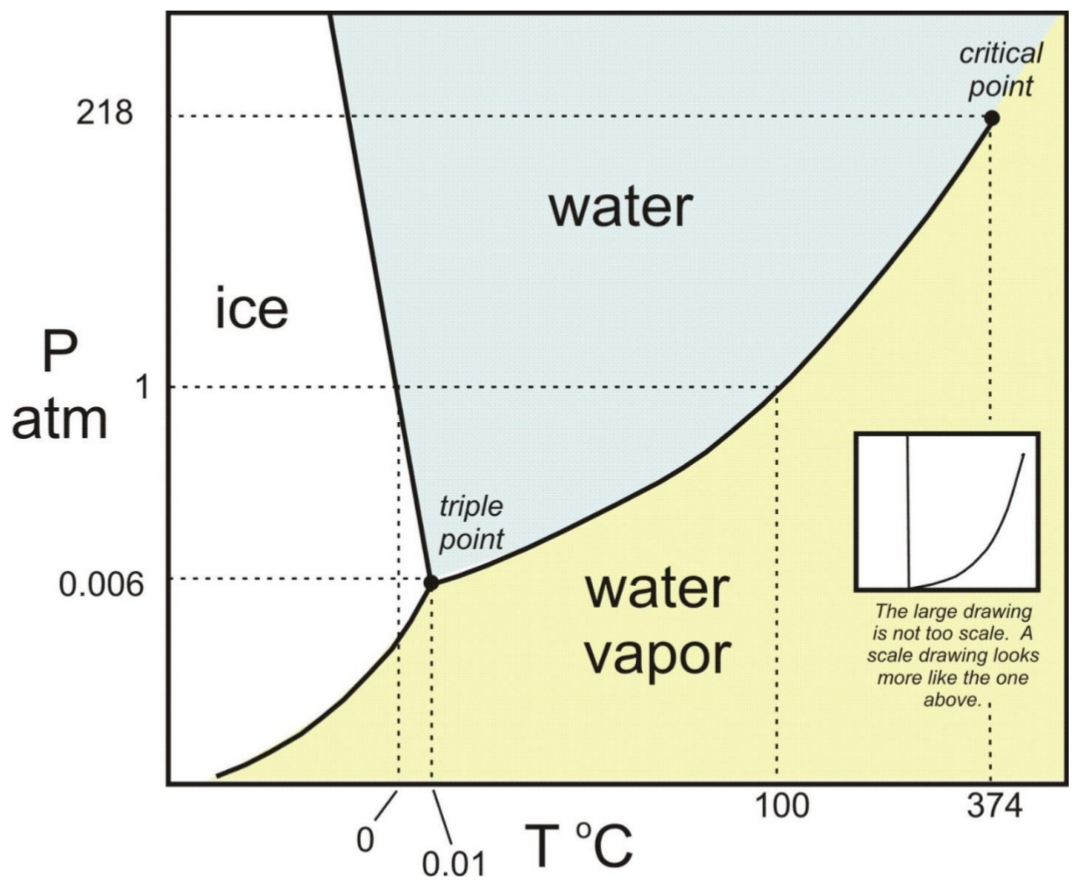
\includegraphics[width=0.7\linewidth]{img/wasser_aggregatszustaende}
	\caption{Aggregatzustände von Wasser}
	\label{fig:wasseraggregatszustaende}
\end{figure}


%-----------------------------------------------------------------------------
\section{TODO}
%-----------------------------------------------------------------------------


Druckabfall Rohrleitung: $\Delta p = \lambda(Re) \frac{\rho u^2}{2}\frac{l}{d}$

$Re = \frac{\rho u d}{\mu}$

$\mu$ = Viskosität

$\rho$ = Dichte

Zähigkeit = dynamische Viskosität


Laminare oder Turbulende ströhmung? 
Re < 2340 -> Laminar
	$\lambda(re) = 64/Re$
	
Re > 2340: Turbulent
	$\lambda(Re) = \frac{0.316}{Re^{1/4}}$

\subsubsection{Einheit Mol}

1 mol Wasser wiegt 18g.

\subsubsection{Allgemeine Gaskonstante}

\[
	N_A k_B = 8.314 \frac{J}{mol \cdot K}
\]

\subsubsection{Klassifizierung thermodynamische Systeme}

Was tauscht ''eine Box'' mit der Umgebung aus?


\begin{description}
	\item[Offen] Tauscht mit der Umgebung Energie und Masse aus
	\item[Geschlossen] Tauscht Energie mit Umgebung aus
	\item[Abgeschlossen] Kein Austausch mit UMgebung
	\item[Adiabatisch] Tauscht mechanische Arbeit mit der Umgebung aus (aber keine Wärme)
\end{description}

\subsubsection{Thermodynamische Begriffe}

\begin{description}
	\item[Thermodynamisches System] Abstraktion für ein reales System, welches Untersucht werden soll, Beispiele: Gastank, Ofen, die Erde
	\item[Thermodynamische Zustandsgrössen definieren das System] Druck, Stoffmenge (Anzahl Moleküle oder Anzahl Mol), Temperatur
	\item[Prozessgrössen beschreiben Prozesse] Wärme und Arbeit
	\item[Wärmelehre oder Thermodynamik] Alles was mit Wärme und Temperatur zu tun hat
	\item[Statistische Mechanik] Herleitung der Thermodynamik aus mikroskopischen Überlegungen, z.B. kinetische Gastheorie
\end{description}


\subsubsection{Zustandsgleichung: Druck, Temperatur, Volumen}


\[
	f(p, T, V) = 0
\]



\[
p V = N k_B T
\]


\begin{description}
	\item[$p$] Absolutdruck
	\item[$V$] Volumen	
	\item[$N$] Anzahl Molekühle
	\item[$T$] Temperatur in Kelvin
	\item[$k_B$] Wolfsmannkonstante
\end{description}

Zustandsgleichung: $\frac{pV}{T} = const.$

%TODO: Slide 5,6


$n$: Molzahl



%-------


\paragraph{Der erste Haptsatz der Thermodynamik:}

Energierhaltung $dU = \delta Q + \delta W$

\begin{description}
	\item[$U$] Innere Energie
	\item[$Q$] Wärme
	\item[$W$] Arbeit
\end{description}

\paragraph{Zweiter Haptsatz:}

Entropie kann nicht abnehmen.

\subsection{Wärmekapazität}

\[
	\delta Q \sim dT
\]

\subsubsection{Beispiel Wärmekapazität}

Wärmekapazität Wasser: $4.1868 kJ / kg K$

Wie viel Energie brauchen wir um 1g Wasser um $1^\circ$ C aufzuwärmen?
%TODO: Beispiel von Slide 19.
\[
SQ = 
\]





\subsubsection{Äquipartitionstheorem}

Wärmekapazität = 0.5 x Anzahl Freiheitsgrade x N x $k_B$

$C = \frac{f}{2}N k_B = \frac{f}{2} nR$

$C_m = \frac{f}{2} R$

$N$ Anzahl Atome


Körper mit gleicher Molzahl haben die gleiche Wärmekapazität


Bei kristalliner Festkörper:

Hohe Temperaturen: $C_{mv} = 3R$

Tiefe Temperaturen %TODO: Slide 24 Formel $C_{mv} = $

\paragraph{Gase}

Bei Gasen wird auch ein Teil der Aufwärm-Energie genutzt, um sich auszudehnen (falls möglich.)




\subsubsection{Phasenübergänge: Thermodynamische Phasen}

\begin{description}
	\item[Fest] Form und Volumen bestimmt
	\item[Flüssig] Bestimmtes Volumen
	\item[Gasförmig] Weder Form noch Volumen bestimmt.
	\item[(Plasma)] Ionisiertes Gas.
\end{description}

%TODO: Grafik seite 33

\subsubsection{Latente Wärme}


\[
Q_f = C_v \Delta T
\]


Bei einem Phasenübergang wird sehr viel Wärme aufgenommen oder abgegeben:

$ \frac{Q_s}{c_v}$

%todo: Tabelle Seite 39



\subsubsection{Dampfdruck}


Der Dampfdruck stellt sich ein, wenn Wasser und Luft im Gleichgewicht sind.

100\% Luftfeuchtigkeit bedeutet: $T = 20^\circ C \Rightarrow P_w = 23.4$ mbar Partialdruck


\subsubsection{Taupunkt}

Bei welcher Temperatur wäre die Luftfeuchtigkeit 100\%?


\subsubsection{Wärmeleitung}
Gesetz von Fourier: Nur Wärme, keine Masse

\paragraph{Wärmestromdichte} $j_Q = - \lambda \frac{dT}{dx}$


$[j_a] = \frac{W}{m^2}$


$[j] = \frac{W}{m^2}$

$[\lambda] = \frac{W}{m \cdot K}$

\paragraph{Wärmeleitungsgleichung} %TODO: Slide 4

\subsubsection{Wärmeübergang - Konvektion}
Wärme + Masse

Die Temperatur ändert sich sehr schnell in einer Grenzschicht. Dafür ist die Konvektion zuständig.

$j = \alpha (T_w - T)$

Wärmeübergangszahl $\alpha$

\paragraph{Beispiel: Wärmeleitung in einem elektronischen Bauteil}
%TODO: Slide 14




\subsubsection{Strahlung}
Stephan-Boltzmann


Jeder Körper > 0 K verliert Energie in Form von elektromagnetischer Strahlung

Die Strahlung ist proportional zu $T^4$ (Stefan-Boltzmann). Die Frequenzverteilung ist eine eindeutige Funktion der Temperatur (Planksches Strahlungsgesetz).

\paragraph{Strahlungsformel von Plank}

Planksche Konstante: $h = 6.626 \cdot 10^-43$

\[
	u(v,T)dv = \frac{hv}{e^{hv/k_BT} - 1} \frac{8\pi}{c^2} v^2 dv
\]

\begin{description}
	\item[$u$] Energiedichte in $\frac{J}{m^3}$
	\item[$v$] Frequenz
	\item[$T$] Temperatur
\end{description}

Atome können nur endliche Quentaen aufnehmen: $e_v = hv$


\paragraph{Elektromagnetische Strahlen}

Können alle perfekt mit der Maxwell-Gleichung beschrieben werden


Die Energie eines Photons: $E_{ph} = hv$. Bei Strahlung, welche Atome zerstören können, nennt man Ionisierende Strahlung.




\paragraph{Stefan-Boltzmann Gesetz}

Bei einer gewissen Temperatur, wie viel Energie geht mit der Fläche verloren.

$\sigma_{SB}$ ist die Stefan-Boltzmann Konstante: $=5.67 \cdot 10^-8 \frac{W}{m^2 K^4}$

Das totale Emissionsvermögen eines schwarzen Körpers ist:

\[
	K_s(T) = \sigma_{SB} T^4
\]

z.B: Wie warm wird eine Herdplatte: $P = \sigma_{SB} \cdot T^4 \cdot A$

 
\subsubsection{Entropie}

In einem geschlossenen System, bei dem das Volumen des Gases grösser wird, ändert sich der Druck. Die Temperatur ändert sich nicht.

$pV = nRT$ bei einem Idealen Gas

$U = \frac{3}{2} nRT$


\paragraph{Eigenschaften der Entropie}

Wärmezufuhr / Temperatur:
\[
	dS = \frac{dQ}{T}
\]

\subsubsection{Hauptsätze der Thermodynamik}

\begin{enumerate}
	\item Energierhaltung
	\item In einem geschlossenen System kann die Entropie nie abnehmen.
\end{enumerate}


\subsubsection{Wirkungsgrad}

Carnot-Wirkungsgrad:

\[
	\eta = 1 - \frac{T_L}{T_H}
\]



\end{document}